\documentclass[aspectratio=169,11pt]{beamer}

\usetheme{Madrid}
\usecolortheme{default}
\usefonttheme{professionalfonts}
\setbeamertemplate{navigation symbols}{}
\setbeamertemplate{footline}[frame number]

\usepackage{amsmath, amssymb, booktabs, graphicx}
\graphicspath{{../../assets/figures/}{assets/figures/}}

\title{Inequality and Wage Dispersion}
\subtitle{Labor I --- Week 8}
\author{Teaching deck draft}
\date{}

\begin{document}

\begin{frame}
  \titlepage
\end{frame}

\begin{frame}{Central question and why this week is heavier}
\begin{itemize}
    \item Week 8 asks how labor economists should measure inequality and organize the mechanisms behind wage and earnings dispersion.
    \item This week is heavier because it consolidates Weeks 1--7 and sets up Weeks 9--10.
    \item We need to separate measurement objects, descriptive decompositions, causal mechanisms, and welfare interpretation.
\end{itemize}
\end{frame}

\begin{frame}{Bridge from Weeks 5--7}
\begin{itemize}
    \item Week 5: wages reflect skill, sorting, and sometimes rents.
    \item Week 6: households transform wage opportunities into hours, earnings, and participation.
    \item Week 7: jobs are wage-plus-amenity bundles, so wage inequality is not automatically welfare inequality.
\end{itemize}
\end{frame}

\begin{frame}{Inequality objects}
\small
\begin{tabular}{p{0.19\linewidth} p{0.31\linewidth} p{0.38\linewidth}}
\toprule
Object & What it captures & What it misses \\
\midrule
Hourly wages & Wage-setting and skill prices & Hours, employment, amenities \\
Annual earnings & Wages plus work quantity & Nonwage job quality \\
Hours / employment & Quantity margins & Wage-setting itself \\
Total job value & Wages plus amenities and stability & Hard to observe directly \\
Household income & Pooling and transfers & Individual labor-market mechanisms \\
\bottomrule
\end{tabular}
\end{frame}

\begin{frame}{Distributional objects}
\[
q_t(\tau) = F_t^{-1}(\tau), \qquad D_t^{90-10} = q_t(0.9) - q_t(0.1)
\]

\begin{itemize}
    \item Quantile gaps let us separate upper-tail and lower-tail inequality.
    \item \(p90-p50\) and \(p50-p10\) answer different questions.
    \item Variance objects and top shares emphasize different parts of the distribution again.
\end{itemize}
\end{frame}

\begin{frame}{Percentile-gap series}
\begin{center}
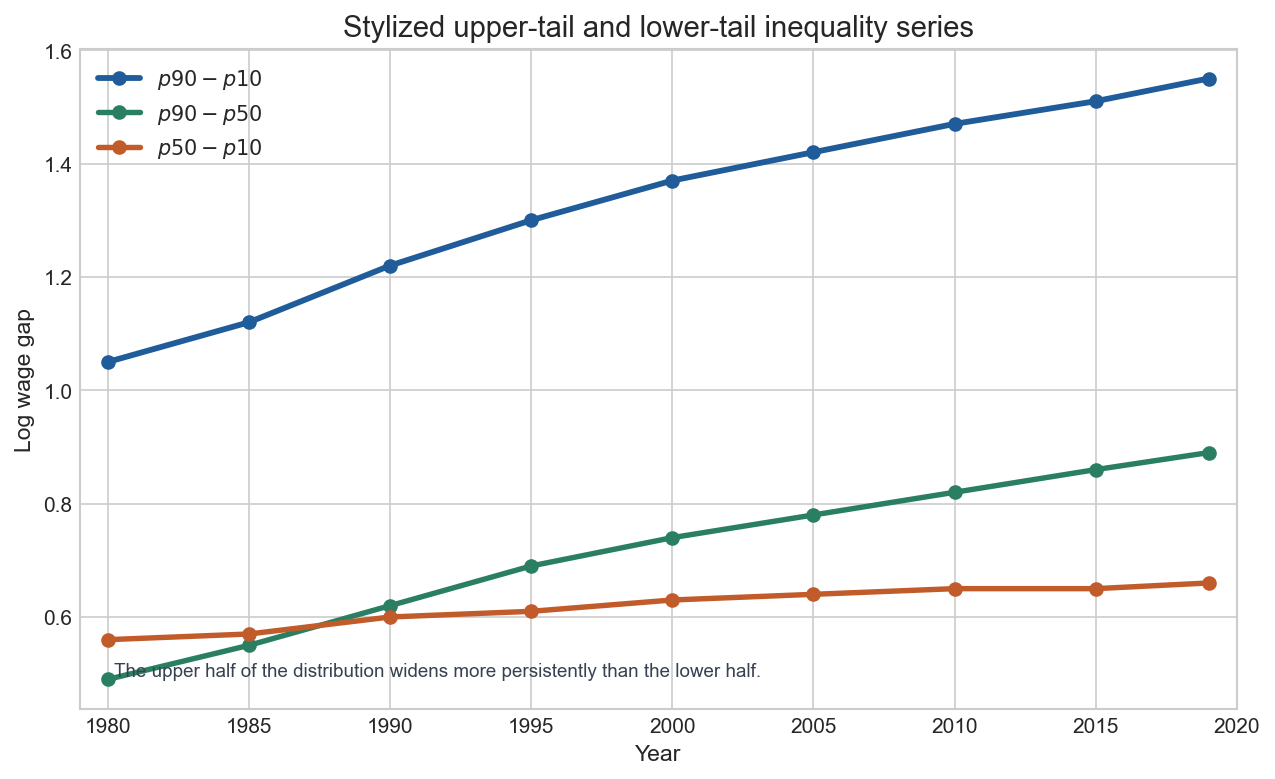
\includegraphics[height=0.74\textheight,keepaspectratio]{08-percentile-gap-series.png}
\end{center}
\end{frame}

\begin{frame}{Between-group versus within-group inequality}
\[
\operatorname{Var}(\log w) =
\operatorname{Var}\!\left(\mathbb{E}[\log w \mid g]\right)
+ \mathbb{E}\!\left[\operatorname{Var}(\log w \mid g)\right]
\]

\begin{itemize}
    \item Inequality can rise because observed group means diverge.
    \item It can also rise because dispersion within groups increases.
    \item This is descriptive accounting, but it strongly disciplines mechanism choice.
\end{itemize}
\end{frame}

\begin{frame}{Residual inequality object}
\[
\log w_{it} = X_{it}'\beta_t + u_{it}
\]

\begin{itemize}
    \item Observable characteristics explain only part of dispersion.
    \item The residual is not one structural force; it mixes unobserved skill, rents, institutions, and measurement limits.
    \item Juhn-Murphy-Pierce made this residual component central to the inequality conversation.
\end{itemize}
\end{frame}

\begin{frame}{Canonical distributional facts}
\begin{itemize}
    \item Upper-tail inequality rises strongly after 1980.
    \item Lower-tail changes are more episodic and institution-sensitive.
    \item The college premium rises, but it is not the entire story.
    \item Composition-adjusted and raw changes need to be distinguished.
\end{itemize}
\end{frame}

\begin{frame}{Tasks and polarization}
\begin{center}
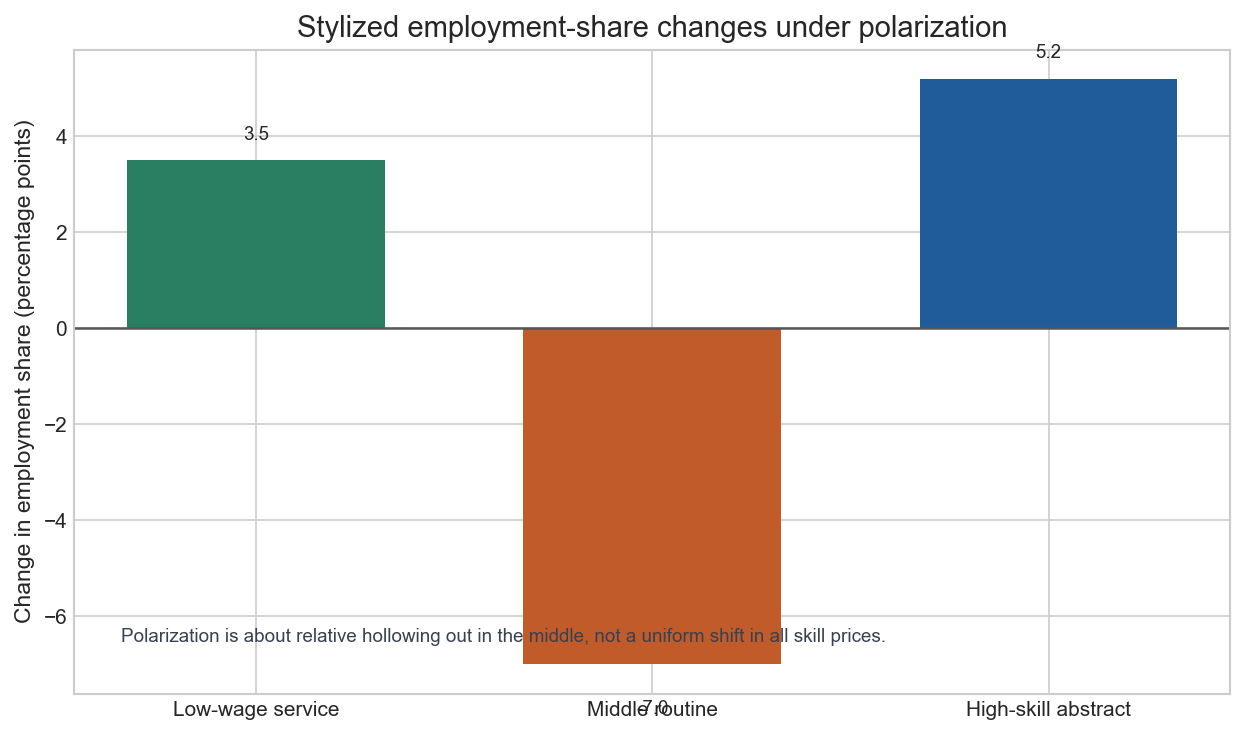
\includegraphics[height=0.74\textheight,keepaspectratio]{08-polarization-schematic.png}
\end{center}
\end{frame}

\begin{frame}{Supply, demand, and skill-premium logic}
\begin{itemize}
    \item Relative demand shifts can raise the return to skill when supply does not keep up.
    \item This logic connects Week 4 human capital directly to Week 8 inequality.
    \item It is strongest for broad skill premiums, but weaker as a complete explanation for every tail of the distribution.
\end{itemize}
\end{frame}

\begin{frame}{Institutions and the lower tail}
\begin{itemize}
    \item Minimum wages, unions, and wage-setting rules often matter most for the lower tail and middle.
    \item Institutional compression changes some percentiles more than others.
    \item Counterfactual distribution work helps separate composition from institutional environments.
\end{itemize}
\end{frame}

\begin{frame}{Firms, rents, and sorting}
\[
\log w_{it} = \alpha_i + \psi_{J(i,t)} + X_{it}'\beta + \varepsilon_{it}
\]

\begin{itemize}
    \item Modern linked employer-employee data adds the employer as an explicit source of wage dispersion.
    \item Inequality can reflect worker heterogeneity, firm premia, and positive sorting between them.
    \item Firm inequality is one way of understanding worker inequality, not a separate topic.
\end{itemize}
\end{frame}

\begin{frame}{Conceptual inequality decomposition}
\begin{center}
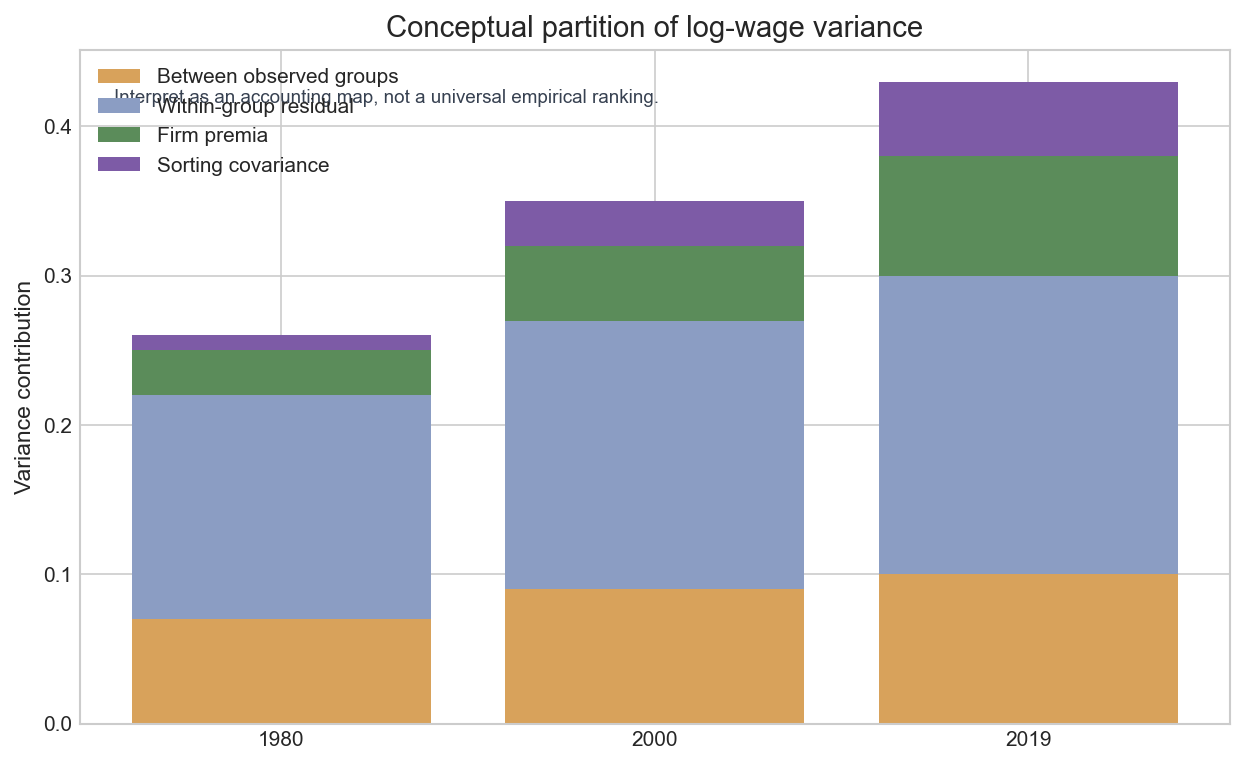
\includegraphics[height=0.74\textheight,keepaspectratio]{08-inequality-component-decomposition.png}
\end{center}
\end{frame}

\begin{frame}{Wages versus total labor-market value}
\[
v_i = w_i + a_i
\]

\begin{itemize}
    \item \(a_i\) captures amenities, safety, schedule quality, stability, or other nonwage job value.
    \item Wage inequality can understate or overstate inequality in total labor-market value.
    \item This is the Week 7 to Week 8 bridge.
\end{itemize}
\end{frame}

\begin{frame}{Wage ranking versus total job value}
\begin{center}
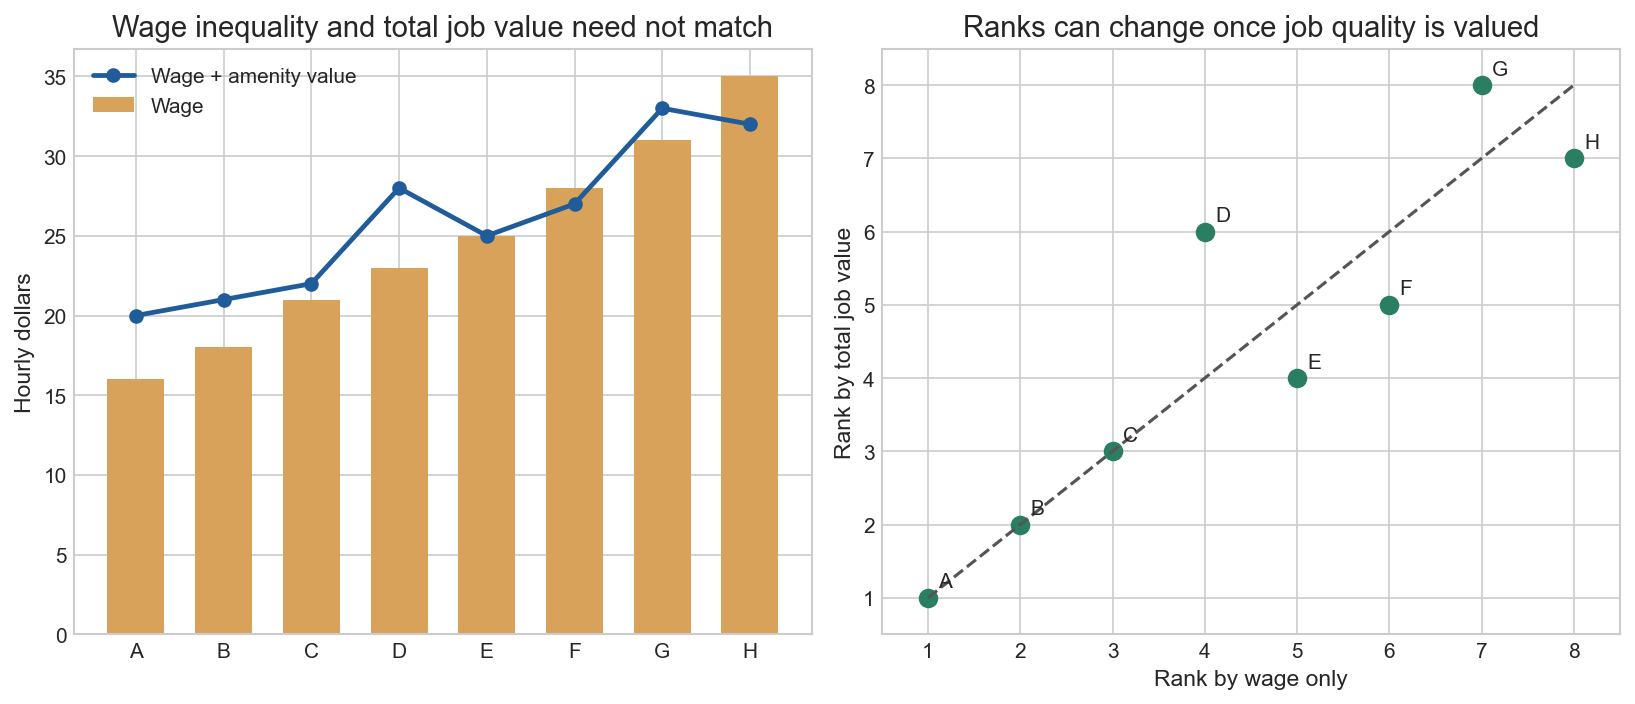
\includegraphics[height=0.74\textheight,keepaspectratio]{08-wage-vs-total-job-value.png}
\end{center}
\end{frame}

\begin{frame}{Empirical toolkit map}
\scriptsize
\begin{tabular}{p{0.18\linewidth} p{0.24\linewidth} p{0.21\linewidth} p{0.25\linewidth}}
\toprule
Method & Main use & Data need & Main limit \\
\midrule
Percentile series & Track distributional change & Repeated wage data & Descriptive only \\
JMP residual decomposition & Separate observables and residuals & Rich micro covariates & Residual mixes mechanisms \\
DFL reweighting & Counterfactual distributions & Cross-sections with overlap & Still partly descriptive \\
RIF methods & Unconditional quantile effects & Micro data plus IF methods & Interpretation depends on functional \\
AKM decomposition & Worker, firm, sorting terms & Linked worker-firm panel & Mobility and design sensitivity \\
\bottomrule
\end{tabular}
\end{frame}

\begin{frame}{Bridge to Week 9}
\begin{itemize}
    \item Group gaps in Week 9 sit inside this wider distributional architecture.
    \item Discrimination is not the same thing as general dispersion in wages, firms, tasks, or places.
    \item Segmentation can operate through amenities and access to high-premium firms as well as through posted pay.
\end{itemize}
\end{frame}

\begin{frame}{Takeaways}
\begin{itemize}
    \item Inequality is multi-object: wages, earnings, employment, and total job value can diverge.
    \item Quantile gaps, variance decompositions, and firm decompositions answer different questions.
    \item No single mechanism explains the post-1980 distribution.
    \item Week 8 is the architecture week for reading discrimination, mobility, and frontier inequality work carefully.
\end{itemize}
\end{frame}

\appendix

\begin{frame}{Appendix: optional extension block}
\begin{itemize}
    \item Linked employer-employee data and AKM implementation details.
    \item Structural interpretations of firm premia, rents, and imperfect competition.
    \item Supply, institutions, and firms across the full wage distribution.
\end{itemize}
\end{frame}

\end{document}
